\chapter{Methodology}

\section{Algorithms}

I have modified \ac{A3C} algorithm in order to take advantage of sub-task with the purpose of enhancing training speed
and exploration.
I refer to this new algorithm \acf{MA3C} and in this section you will find specifications about the architectures of
both \acp{NN}: \ac{A3C} and \ac{MA3C}.
In addition I will explain the \ac{MA3C} algorithm.

They have been developed using tensorflow (\cite{tensorflow2015}), an open source machine learning framework which I find
really useful to implement deep learning algorithms.

\subsection{\acl{A3C}}

As I explained previously (\ffref{subsec:A3C}) this algorithm uses the image of the environment to represent the state.
I have used almost the same preprocessing and network architecture (\ffref{fig:A3C}) than in \citetitle{sutton1998introduction} (\cite{mnih2013}).
In practice the images of any game are downsampled to $84 \times 84$ grayscale pixels in order to reduce the computational cost of training,
specifically the input dimensionality.
The algorithm applies this preprocessing to 4 stacked frames allowing the neural network to calculate (implicitly) the movement
of the different pixels/ objects on the screen.
The state dimensionality is $84 \times 84 \times 4$ which defines the input layer of the \ac{DNN}.

There are several hidden layers specifically designed for obtaining high level abstractions of the environment frames.
The first one is a convolutional layer (\ffref{subsec:CNN}) with $16$ filters with kernel dimension $8 \times 8$ and stride $4$,
followed by a \ac{ReLU} layer.
The second layer is also a convolutional layer, but with $32$ filters with kernel dimension $4 \times 4$ and stride 2,
again followed by a \ac{ReLU} layer.
The last hidden layer intends to represent general features about the state of the game.
It is a fully connected composed by 256 ReLU nodes.

From this 256 features the actor and critic layers, which are the output layers, decide the actions that should be taken
in order to maximize the reward, as explained in (\ffref{subsec:AC}).
The actor is made up by as many nodes as actions available in each game with values from $0$ to $1$, representing the
probability distribution $\pi$.
The critic is just $1$ neuron representing the value function $V(s_t)$.

\begin{figure}[hbtp]
\begin{center}
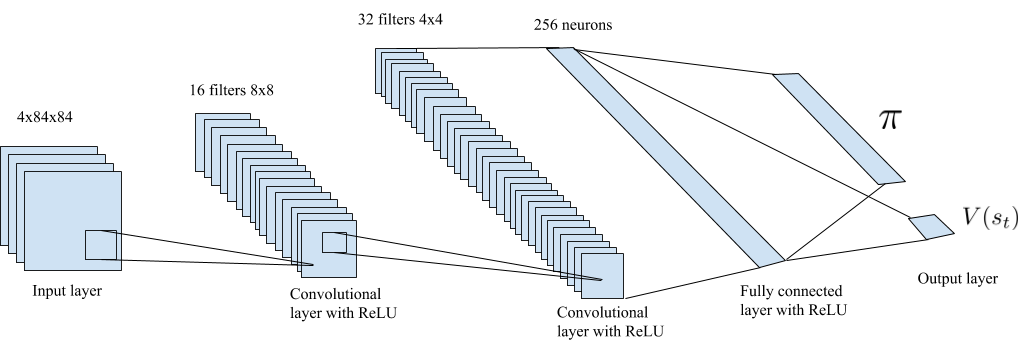
\includegraphics[width=430]{img/A3C_architecture.png}
\end{center}
\caption[A3C architecture]
{Architecture of the \ac{A3C} algorithm.}
\label{fig:A3C}
\end{figure}

\subsection{\acl{MA3C}\label{subsec:MA3C}}

This algorithm is strongly associated with hierarchial reinforcement learning, since the last layer of \ac{A3C}
($\pi and \V(s_t)$) is replicated several times in order to model different tasks inside a common bigger problem.
% TODO EXPRESAR LOS PROBLEMAS COMO OPCIONES?
% TODO HACE FALTA REPLICAR V(S)?

\section{Environments}
The ultimate goal of this thesis is to play Montezuma's revenge, but since it is a complex game i have developed two
simpler environments.
Both helped me to understand the pros and cons of \ac{A3C} and to develop a new version of this algorithm that uses subtasks.

\subsection{Simple States}

This game is made by a $6 \times 10$ grid of square blocks.
Their colors define the kind of object and how they will interact with the hero (an special object).
This are the different types:
\begin{itemize}
  \item \newconcept{hero}: A block that can be controlled by the actions.
  \item \newconcept{wall}: If the hero hits a wall the game ends and he obtains a reward of value -1.
  When this happens we say that the hero dies.
  \item \newconcept{checkpoint}: When the hero reach this object he obtains a reward of value 1 and enables the hidden
  checkpoint reward.
  Once the hero reaches it for the first time he will never obtain the reward again.
  \item \newconcept{hidden checkpoint}: When the hero reach this object enables the door.
  It basically forces the hero to pass and there is no reward when this happens.
  \item \newconcept{door}: If the hero reach the door having gone through the different checkpoints the game ends and
  he obtains a reward of value 1.
\end{itemize}

\begin{figure}[hbtp]
\begin{center}
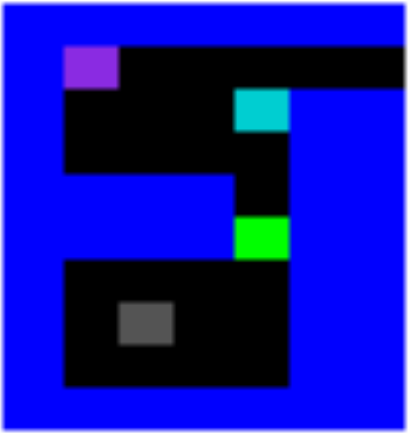
\includegraphics[width=200]{img/SimpleStates_going_up.png}
\end{center}
\caption[Simple States game]
{The hero navigating through a hostile environment trying to reach the door. The wall, hero, checkpoint, hidden checkpoint
and door are represented with the following colors respectively: blue, grey, green, turquoise and violet}
\label{fig:SimpleStates}
\end{figure}

As you can imagine the goal of the hero is to reach the door by going through the different checkpoints without colliding
with any wall, the maximum score is 2.
The game is organized in three different phases/states.
The objective of the first one is to reach the checkpoint,
the second one the hidden checkpoint and the third one the door.
The information about the current phase is available
to the player.

The purpose of creating this game is to prove that the \ac{MA3C} algorithm (\ffref{subsec:MA3C}) has better exploration
skills than A3C (\ffref{subsec:A3C}).

\subsection{Complex States}
This game is really similar to the previous one but the dynamics are a bit different.
The hero must follow a series of steps to reach the door.
The order in which the hero must go through the objects is: checkpoint, hidden checkpoint, door, hidden checkpoint,
checkpoint, door.
We force the hero to go back on his own steps when he reaches the door.
In this game some of the rewards also change.
This are the changes respect to Simple States game, the rest remains equal:
\begin{itemize}
    \item \newconcept{checkpoint}: The first time that the hero goes through this object he obtains a reward of 1.
    Then he must follow the rest of the path described above to obtain again 1 of score (after the second time he visits the hidden checkpoint).
    \item \newconcept{hidden checkpoint}: In this game both 2 times that the hero goes through this object
    (following the path) receives 1 of score.
    The first time the checkpoint object enables the reward and the second time the door enables it.
    \item \newconcept{door}: The first time the hero reach the door it moves to the starting position of the hero (bottom left corner)
    and gives him 1 of score.
    The second time behaves as in Simple States.
\end{itemize}

\begin{figure}[hbtp]
\begin{center}
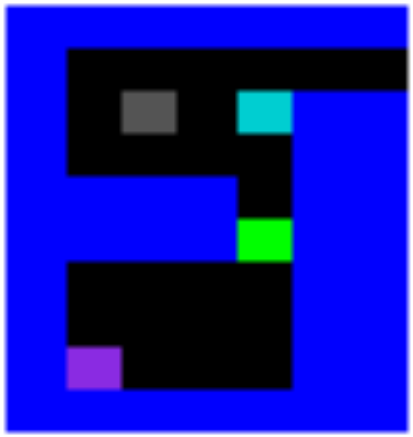
\includegraphics[width=200]{img/ComplexStates_going_back.png}
\end{center}
\caption[Complex States game]
{The hero after reaching the door for first time. The wall, hero, checkpoint, hidden checkpoint
and door are represented with the following colors respectively: blue, grey, green, turquoise and violet}
\label{fig:ComplexStates}
\end{figure}


In this game there are only two phases.
The first one goes from the start until the first time the hero reaches the door.
The second one finish the second time it reaches the door.
As in Simple States the hero must follow the path in order to obtain the rewards and finish the game.
The information about the current phase is also available to the player.

The purpose of creating this game is to prove that \ac{A3C} is quite bad going back on his own steps (when the image of the
game is similar) while for \ac{MA3C} is easy.
%%% Local Variables: 
%%% mode: latex
%%% TeX-master: "../report"
%%% End: 
